\section{Програмная реализация}
В качестве языка для реализации работы\footnote{https://github.com/hawkeoni/Thesis} был выбран Python 3.6. Данный язык позволяет быстро разрабатывать простые сервисы и имеет ряд библиотек для работы с нейросетевыми моделями. В качестве фреймворка для глубокого обучения используется Pytorch 1.6.0 и библиотека AlenNLP 1.1.0.

Кодовую базу можно разделить на несколько модулей:

\begin{itemize}
    \item Модуль обработки корпусов (800 строк) - данный код отвечает за обработку текстовых коллекций в форматы для обучения. Исходные форматы корпусов в форматах CSV, JSON, XML, MySQL dump были преобразованы в человекочитаемый формат JSONL.
    \item Модуль моделей (500 строк). В данном модуле написаны нейросетевые архитекутры и классы для взаимодействия с ними.
    \item Модуль обучения (500 строк). В данном модуле написаны циклы обучения, подсчет метрик, интеграции с системой отслеживания экспериментов\footnote{https://wandb.ai/hawkeoni}.
    \item Веб-сервис (250 строк) - реализован стенд для удобного взаимодействия с моделями на микрофреймворке Flask 1.1.1.
\end{itemize}

Выбор библиотек Pytorch и AllenNLP обоснован их простотой и возможностью быстрого прототипирования нейросетевых архитектур. Выбор микрофреймворка Flask для веб-сервиса был сделан из-за возможности легко создать веб-приложение на несколько страниц для взаимодействия с моделями.

Обучение происходило удаленно на сервере DataCrunch\footnote{https://datacrunch.io/} с видеокартами Tesla V100 с 16Гб видеопамяти. Процесс обучения в зависимости от корпуса занимал от 30 минут до 8 часов.

\begin{figure}[h!]
\centering
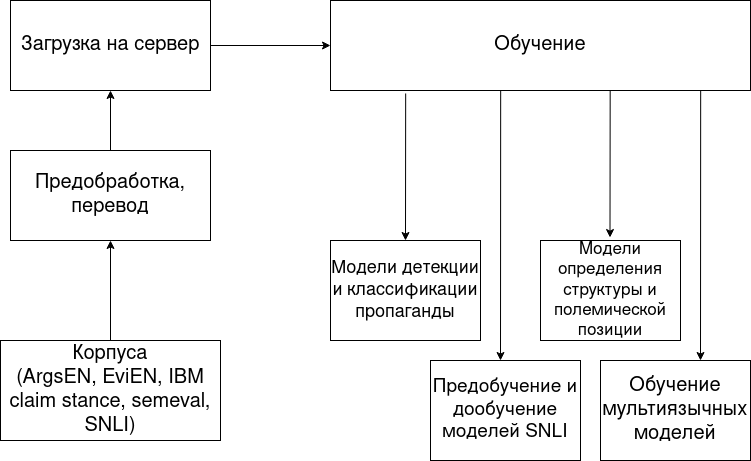
\includegraphics[scale=.5]{Комплекс.png}
\caption{Процесс обучения модели.}
\label{Problem_Picture}
\end{figure}


Для исследования эффективности работы моделей извлечения аргументации было создано веб-приложение. Веб-приложение содержит в себе одну страницу для взаимодействия с моделями. На странице предоставлены поля для компонент аргументации и выбора моделей. После заполнения полей и выбора моделей на странице с помощью языка JavaScript отображается результаты работы моделей определения структуры аргументации (релевантности) и полемической позиции (поддержка или атака).

\begin{figure}[H]
 \captionsetup{justification=raggedright,singlelinecheck=false,labelfont=bf,labelsep=period,name={Рисунок}}
 \centering{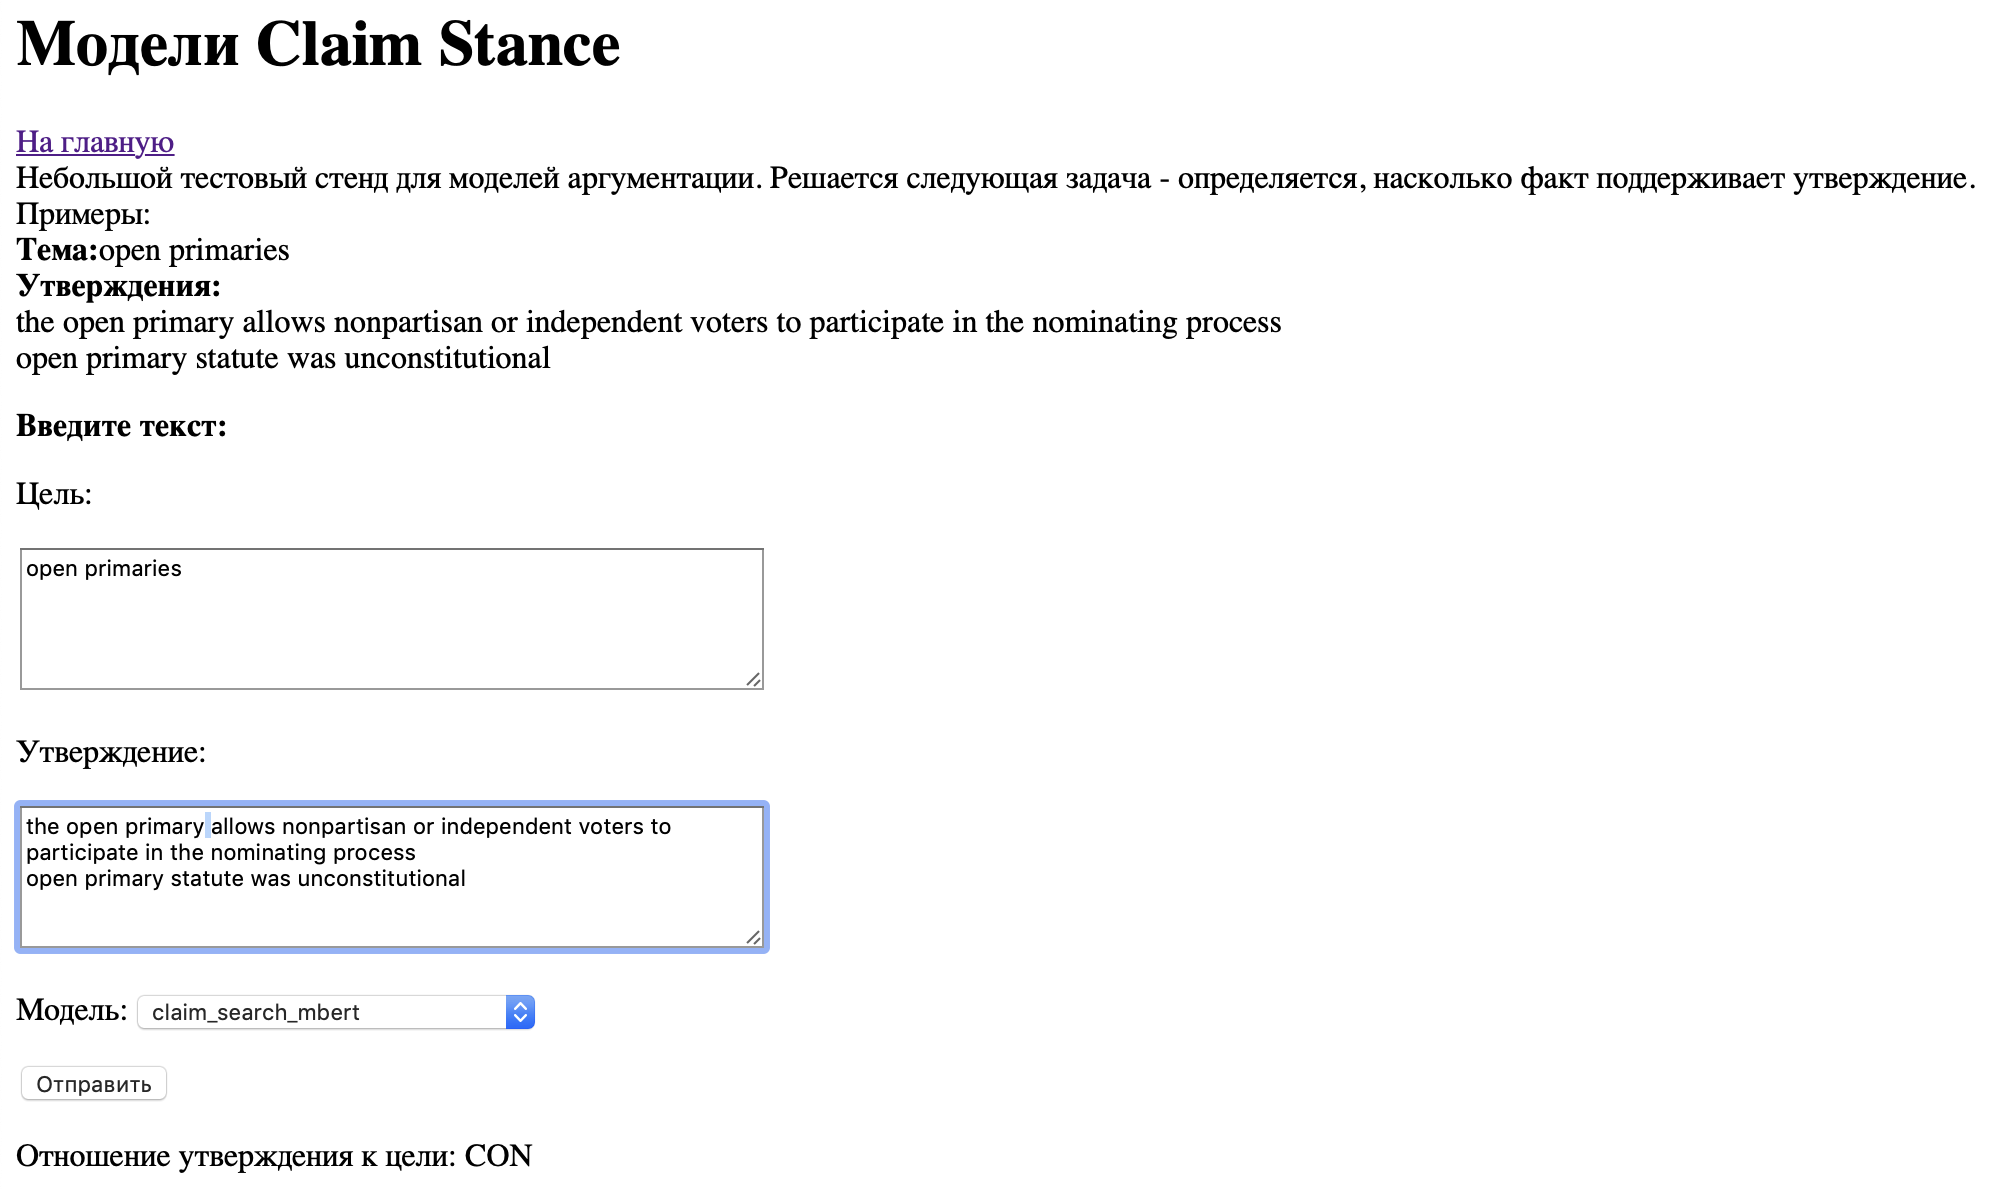
\includegraphics[scale=0.5]{service.png}}
 \caption{Интерфейс сервиса.}
\end{figure}



\begin{comment}
\section{Описание практической части}
\subsection{Экспериментальное исследование}

\subsubsection{Выделение предпосылок}

Первый корпус был взят из работы \cite{aharoni2014benchmark}. Данный корпус состоит из размеченных тем и предпосылок. Всего в корпусе представлено 83 темы. В данном корпусе пары размечены бинарным отношением  наличия релевантности, при этом под релевантностью подразумевается исключительно поддержка, т.е. в рамках данной постановки задачи предпосылки, противоречащие утверждению, имеют тот же класс, что и предпосылки, не имеющие никакого отношения к утверждению. Пример утверждения, относящегося к теме:
\begin{verbatim}
Утверждение: We should increase gun control
Обоснование: Gun control laws are depicted as benign and 
historically progressive.
\end{verbatim}

Для исследования возможности переноса знаний между языками данный корпус был переведен на русский язык.

Так как идейно в этой задаче моделируется связь между двумя высказываниями было решено адаптировать корпуса из задачи Textual Entailment (Natural Language Inference). Был адаптирован русскоязычный корпус TERRa, состоящий из гипотез и предпосылок, которые очень близки к предыдущему корпусу. Пример связанной гипотези и предпосылки:
\begin{verbatim}
Предпосылка: Автор поста написал в комментарии, 
что прорвалась канализация.
Гипотеза: Автор поста написал про канализацию.
\end{verbatim}


Было проведено несколько различных экспериментов. Исследовалась переносимость знаний на русский язык и влияние стороннего корпуса на эффективность переноса знаний. Обучение и валидация происходили на англоязычной версии корпуса. Были обучены следующие вариации моделей:
\begin{itemize}
    \item combined\_mbert\_frozen - мультиязычная модель, обученная на корпусе TERRa и корпусе IBM Evidence Search.
    \item ibm\_mbert\_frozen - мультиязычная модель, обученная на корпусе IBM Evidence Search.
    \item terra\_mbert\_frozen - мультиязычная модель, обученная на корпусе TERRa.
\end{itemize}

Как видно из графиков обучения, лучше всего работает модель ibm\_mbert\_frozen. Как и все названные модели она базируется на модели multilingual BERT. При обучении для применения техники crosslingual transfer у модели замораживается матрица эмбеддингов.

На англоязычной тестовой выборке модели показывают F1-меру около 0.75. При переходе на переведенную русскоязычную версию корпуса качество падает до 0.72-0.73, что говорит об успешном переносе знаний.

\begin{figure}[h!]
  \centering
  \begin{minipage}[b]{0.45\textwidth}
    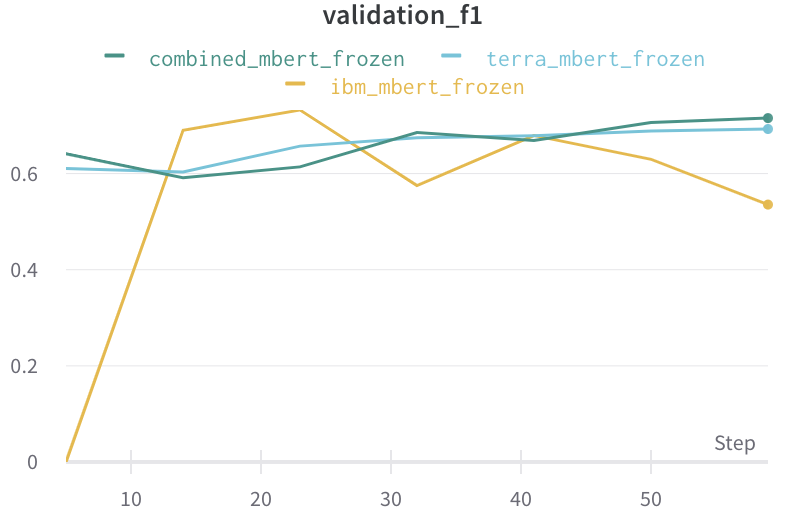
\includegraphics[width=\textwidth]{f1.png}
    \caption{F1-мера на задаче поиска предпосылок.}
  \end{minipage}
  \hfill
  \begin{minipage}[b]{0.45\textwidth}
    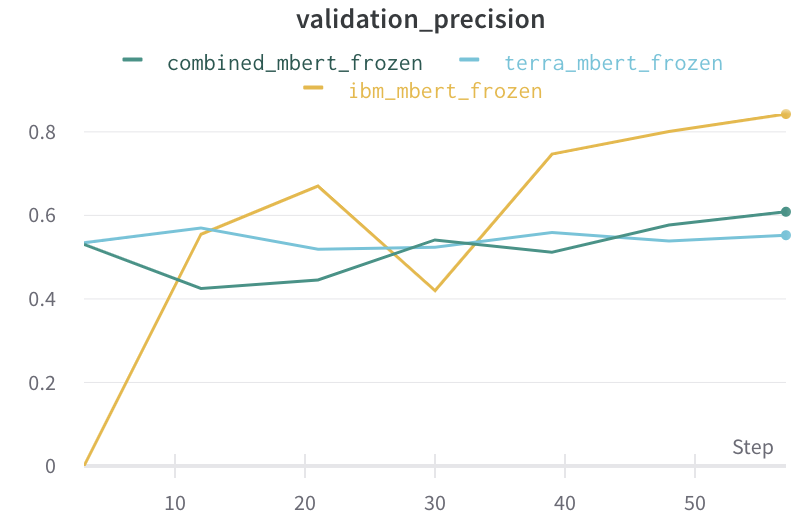
\includegraphics[width=\textwidth]{precision.png}
    \caption{Точность на задаче поиска предпосылок.}
  \end{minipage}
  \begin{minipage}[b]{0.45\textwidth}
    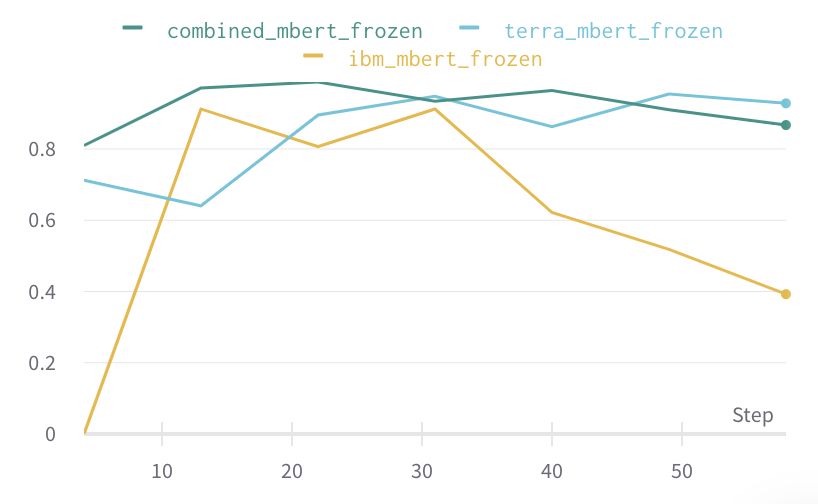
\includegraphics[width=\textwidth]{recall.png}
    \caption{Полнота на задаче поиска предпосылок}
    \label{pd_3}
  \end{minipage}
\end{figure}



Стоит отметить, что на этом корпусе нет установленной таблицы лидеров, поэтому заявленные числа тяжело оценить из-за отсутствия каких-либо конкурентов. Однако ранее упомянутая система MARGOT заявляет об F1-мере в 0.3. Подробные примеры работы можно увидеть в приложении.


\subsubsection{Классификация предпосылок}
У предыдущей постановки задачи существуствует один важный недостаток - она не позволяет различить нейтральную связь от атакующей. Для этого был адаптирован корпус \cite{bar2017stance}, позволяющий определить полемическую позицию аргументации. Под полемической позицеий в данном контексте понимается тип связи между предпосылкой и утверждением или темой. Позиция бывает трех типов: нейтральная, атакующая (опровергающая, противоречащая) и поддерживающая (согласованная). В данном  корпусе размечены аналогичные пары утверждений и предпосылок в отношения атаки и поддержки. В данном корпусе отсутствуют нейтральные отношения. Для этого были дополнительно обработаны исходные тексты, и все тексты, не размеченные в поддержку или атаку считались нейтральными. Пример:
\begin{verbatim}
Утверждение: Реклама вредна
Предпосылка: Реклама распространяет консьюмеризм и культуру потребительства
Вид связи: Поддержка

Утверждение: Бокс полезен
Предпосылка: Бокс остается 8м самым летальным видом спорта
Вид связи: Атака
\end{verbatim}

Вместо задачи бинарной классификации в отношения атаки и поддержки рассматривается задача регрессии в отрезок $[-1; 1]$, где -1 - атака, 1 - поддержка, 0 - нейтральное отношение. Для получения классов данный отрезок был поделен на 3 равные части. По этим частям вышла точность в 62\%.

\begin{figure}[H]
 \captionsetup{justification=raggedright,singlelinecheck=false,labelfont=bf,labelsep=period,name={Рисунок}}
 \centering{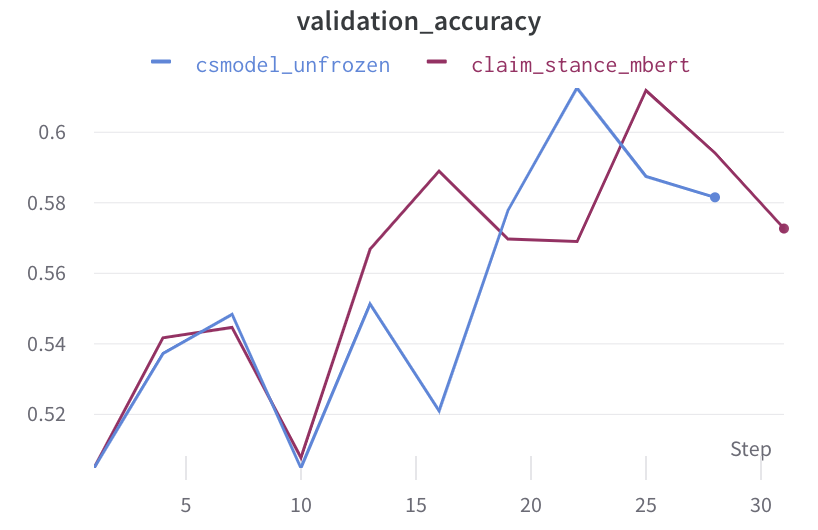
\includegraphics[scale=0.8]{accuracy.png}}
 \caption{Точность системы классификации полемической позиции предпосылок по отношению к утверждениям.}
\end{figure}

Стоит отметить, что в задачах очень сильные сдвиги в распределениях - нейтральных примеров много больше, чем положительных или отрицательных.

\subsubsection{Исследование полученного решения}

С помощью веб-интерфейса проводилось исследование полученных систем. В первую очередь хотелось понять, насколько в модели используется некое внутреннее знание, и насколько в модель опирается на структурные особенности аргумента, такие как общие слова и окрашенную лексику.

Эксперименты показали, что модели улавливает антонимию и отрицания с помощью частицы ``не'', но у модели возникают проблемы со сложными темами, не вошедшими в обучающие корпуса. Проблема данных корпусов в том, что они содержат большое число примеров на ограниченном наборе тем, в то время как в рамках предобученной модели предпочтительнее было бы иметь разнообразное число тем.

\subsection{Обнаружение пропаганды}

Как отмечалось ранее, пропаганда является политической аргументацией, хотя в некоторой литературе ее называют ``ложной'' аргументацией. Было принято участие в соревновании  SemEval 2020 Task 11 Propaganda Detection In News Articles\cite{da2020semeval}. Было представлена два трека - детекция пропаганды и классификация пропаганды. По результатам\cite{dimov-etal-2020-nopropaganda} участия было занято 7 место из 36 в первом треке и 6 из 31 во втором треке.

Корпус состоял из ручной разметки новостных статей за 2019 год. Всего было обработано 438 статей, содержащих 21230 предложений, из которых 7485 содержали пропаганду.

\subsubsection{Определение участков текста с пропагандой}
В первом треке требовалось определить участки текста, являющиеся пропагандой, т.е. постановка задачи заключается в бинарной разметке текста на предмет наличия приемов убеждения. 

\begin{figure}[H]
 \captionsetup{justification=raggedright,singlelinecheck=false,labelfont=bf,labelsep=period,name={Рисунок}}
 \centering{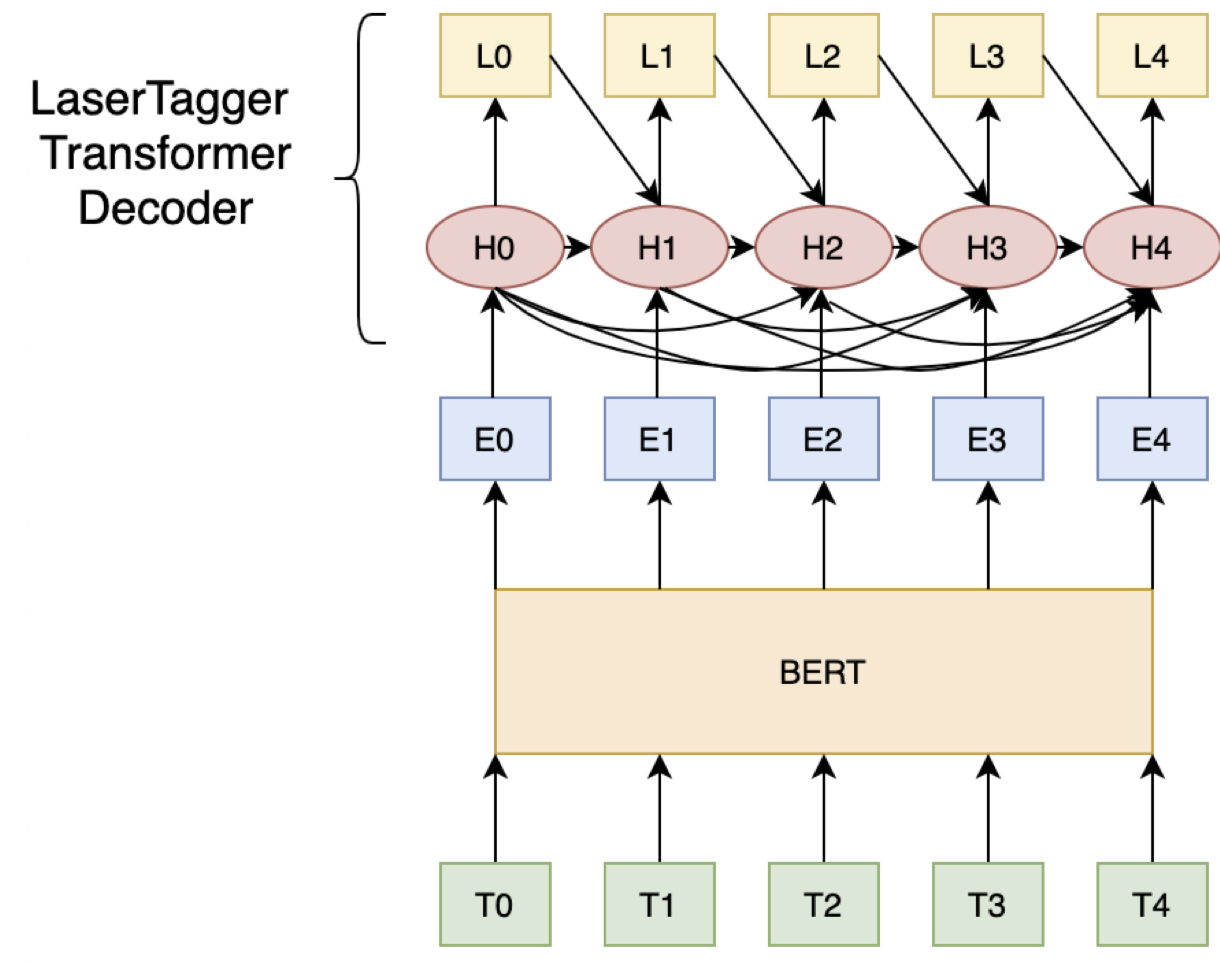
\includegraphics[scale=0.5]{lasertagger.png}}
 \caption{Архитектура LaserTagger из первого трека. $T_i$ - входная последовательность токенов, $L_i$ - бинарные метки для токенов.}
\end{figure}

Т.к. задача тэгирования последовательности, частным видом которой является распознавание именованных суностей, имеет ряд стандартных архитектур, было решено применить несколько стандартных подходов для получения хорошего базового решения.

\begin{figure}[H]
\setcounter{figure}{0}
 \captionsetup{justification=raggedright,singlelinecheck=false,labelfont=bf,labelsep=period,name={Таблица}}
 \centering{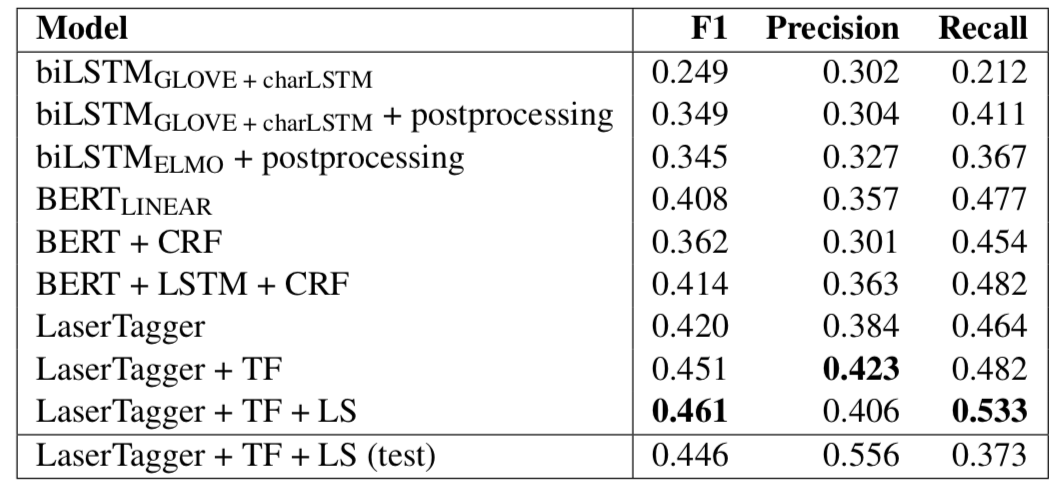
\includegraphics[scale=0.7]{laser_table.png}}
 \caption{Архитектура LaserTagger из первого трека. $T_i$ - входная последовательность токенов, $L_i$ - бинарные метки для токенов.}
\end{figure}

В результате была принята авторегрессионная модель LaserTagger \cite{malmi2019encode}. По сравнению с обычными моделями тэгирования у нее есть одно важное преимущество: она учитывает свои предыдущие предсказания, поэтому она имеет возможность предсказывать длинные непрервыные участки текста без разрывов.

Как видно из таблицы стандартные пододы получают низкие метрики в районе 24-35\% F1-меры. Использование CRF для связного предсказания меток не приносит пользы. Базовая модель, основанная на BERT сразу получает метрику в 40\%.

Для обучения финальной версии архитектуры lasertagger использовалась методика labelsmoothing для смягчения ошибок по краям пропаганды, а также teacher forcing. Teacher forcing заключается в смешивании результатов авторегресионной модели с ее предсказаниями во время обучения. Таким образом получается, что модель ошибается во время обучения и ислледуюет больше пространства и становится более устойчивой к ошибкам.

\subsubsection{Классификация пропаганды}

\cite{wu2019enriching}
Данный трек заключался в классификации участков с пропагандой в один из 18 классов:
\begin{itemize}
    \item Сильно окрашенная лексика. Пример: ".. a lone lawmaker’s childish shouting."
    \item Навешивание ярлыков и имен. Пример: "Republican congressweasels"
    \item Повторение. Заключается в повторении тезиса для закреплении концепции в голове у слушателей.
    \item Преувеличение или приуменьшение. Пример: "Democrats bolted as soon as Trump’s speech ended in an apparent effort to signal they can’t even stomach being in the same room as the president"
    \item Сомнения. Пример: "Is he ready to be the Mayor?"
    \item Взывание к страхам и предрассудкам. Пример: "stop those refugees; they are terrorists"
    \item Сбор под флагом, т.е. взывание к аудитории на почве общей какой-либо общей идентичности (национальности, пола и т.п.). Пример: "entering this war will make us have a better future in our country"
    \item Упрощение причины, т.е. упор на какую-либо первопричину в проблеме с множеством факторов. Пример: "If France had not declared war on Germany, World War II would have never happened."
    \item Слоганы - любые яркие фразы, взывающие к эмоциям. Пример: "Make America great again!"
    \item Диктатура - представление ограниченного выбора в задаче, где существует большее число вариантов решение проблемы. Пример: "There is no alternative to war."
    \item Терминирующие размышления клише - фразы дискредитирующие критичекское размышление по теме обсуждения. Пример: "никто не идеален" или "нельзя изменить человеческую натуру"
    \item Whataboutism - перевод темы для занятия более высокой моральной позиции. Пример: "А у вас права ущемляют!".
    \item Сведение вопроса к заведомо осуждаемой теме. Пример: "Only one kind of person can think this way: a communist!"
    \item Красная сельдь - представление нерелевантной информации для отвращения внимания. 
    \item Стадность - захват мнения через представление позиции, как поддерживаемой большинством. Пример: "Would you vote for Clinton as president? 57\% say yes."
    \item Нарочитая расплывчатость и неясность.
    \item Соломенный человек - подстановка похожего утверждения вместо утверждения оппонента с его последующим опровержением.
\end{itemize}
Классы довольно несбалансированны, поэтому вместо 18 классов для работы модели их число сократили до 14, объединив последние классы в 2 группы. Также стоит отметить, что каждый участок пропаганды может принадлежать более чем одному классу.

\begin{figure}[H]
\setcounter{figure}{12}
 \captionsetup{justification=raggedright,singlelinecheck=false,labelfont=bf,labelsep=period,name={Рисунок}}
 \centering{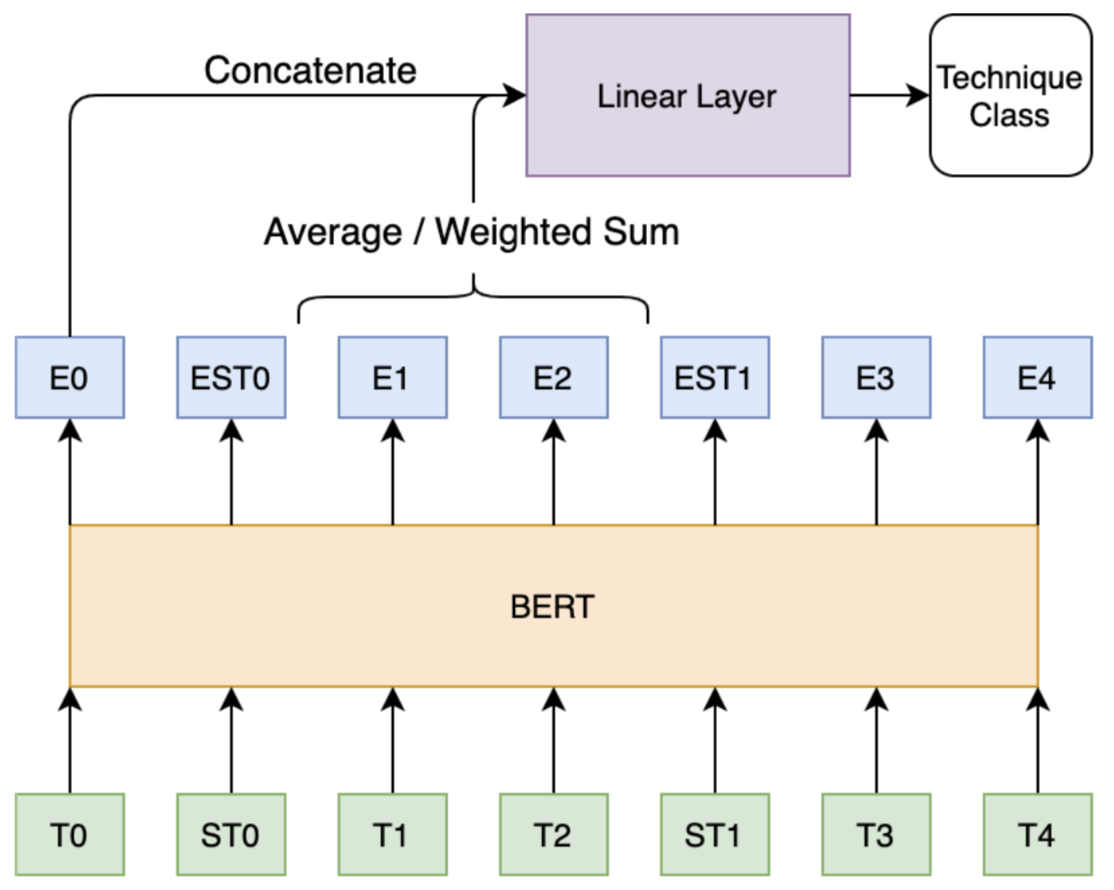
\includegraphics[scale=0.5]{rbert.png}}
 \caption{Результаты моделей классификации пропаганды.}
\end{figure}

Была применена модель RBERT, позаимствованная из задачи извлечения отношений. Особенностью данной модели является обособление участков текста спецсимволами. Также было использовано несколько обычных моделей классификации.

В модели RBERT был использован механизм пулинга через веса, полученные в результате работы механизма внимания.В конечной посылке был использован ансамбль обученных моделей.

\begin{figure}[H]
\setcounter{figure}{1}
 \captionsetup{justification=raggedright,singlelinecheck=false,labelfont=bf,labelsep=period,name={Таблица}}
 \centering{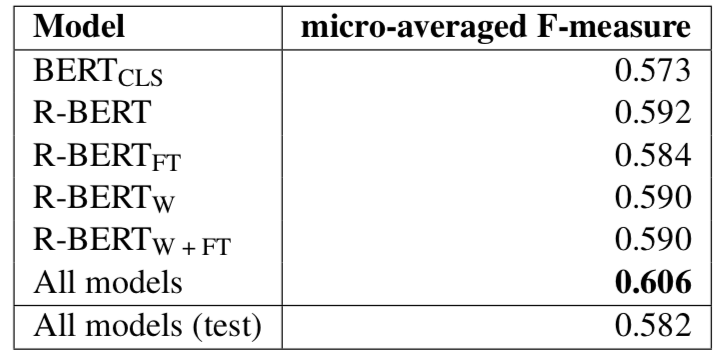
\includegraphics[scale=0.7]{rbert_table.png}}
 \caption{Архитектура RBERT из второго трека. $T_i$ - входная последовательность токенов, $E_i$ - внутреннее представление токенов в модели.}
\end{figure}


\subsubsection{Исследование полученного решения}
Анализ ошибок модели выделения пропаганды показал, что данная модель имеет и некоторые недостатки: модель часто выделяет различные обособленные обороты и цитаты полностью, вместо их частей. Выделение цитат легко объяснить - они очень часто содержат речь, которая более эмоционально и содержит самый частый класс пропаганды. Также модель иногда наоборот закрывает участок с пропагандой при переходе через запятую и не открывает участок заново.

Часть проблем возникает и из-за особенностей корпуса. В корпусе прослеживается сильное смещение тем между тестовой выборкой и тренировочной, валидационной. Из-за этого метрики всех участников на валидационной выборке на 10-15\% выше, чем итоговые результаты на тесте.

Анализ модели классификации выявил, что она хорошо выделяет частотные классы, но хуже справляется с редкими.

Две команды, занявшие первые места в треках, использовали более простые  модели для тэгирования последовательности, однако обе использовали подход активной доразметки других открытых корпусов, что говорит о том, что и предложенные в этой работе системы могут быть улучшены за счет увеличения обучающей выборки.

\subsection{Программная реализация}
Код\footnote{https://github.com/hawkeoni/Thesis.}, сопровождающий данную работу, написан на языке Python 3.6.x и логически разделяется на следующие компоненты с соответствующими объемами:
\begin{itemize}
    \item Логика веб-приложения - обработка запросов и применение моделей. 80 строк кода на языке Python.
    \item Страницы веб-приложения - 100 строк на HTML.
    \item Javascript сценарии для удобного интерфейса веб-приложения - 60 строк.
    \item Код для предобработки данных в формат удобный для обучения из таких форматов как CSV, JSON, XML, MySQL dump - 720 строк.
    \item Код для обучения - нейросетевый модели, преобразование данных в многомерные массивы, логирование метрик, составляет 335 строк.
    \item Код для доступа к онлайн интерфейсам для перевода текстов - 81 строка.
    \item Конфигурационные JSON-файлы для архитектуры моделей и стратегии их обучения - 370 строк.
\end{itemize}

Ради скорости прототипирования для разработки приложения был выбран микро-фреймворк Flask версии 1.1.1. Для написания и обучения нейросетевых архитектур используется связка библиотеки Pytorch\cite{pytorch} версии 1.6.0 и AlleNLP\cite{allennlp} версии 1.1.0. Совокупность данных библиотек позволяет удобным образом писать конфигурации для экспериментов в формате JSONNET. Пример подобного конфигурационного файла можно посмотреть в \hyperref[sec:jsonnet]{приложении}. Большие предобученные языковые модели, такие как \textbf{BERT, ROBERTa, ruBERT} и т.п. были взяты из библиотеки Transformers\cite{transformers} версии 3.0.2.

Прогресс обучения моделей логируется в онлайн-сервисе wandb\footnote{https://wandb.ai/hawkeoni}.

\begin{figure}[H]
\setcounter{figure}{13}
 \captionsetup{justification=raggedright,singlelinecheck=false,labelfont=bf,labelsep=period,name={Рисунок}}
 \centering{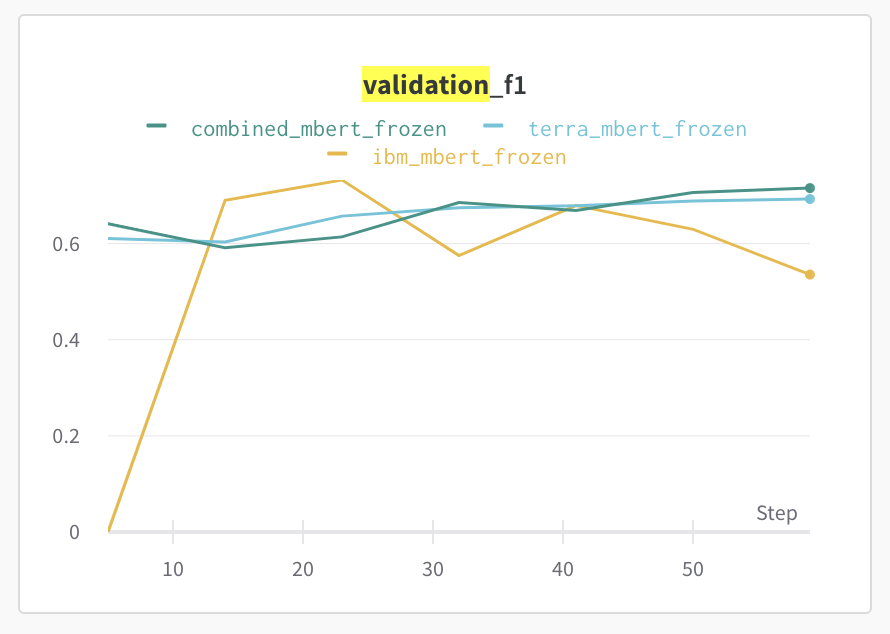
\includegraphics[scale=0.8]{wandb.png}}
 \caption{Пример графика, логируемого в сервис wandb.}
\end{figure}

Дополнительно для удобства веб-приложение собрано в Docker-контейнер.

\subsection{Описание веб-сервиса}
\begin{figure}[H]
 \captionsetup{justification=raggedright,singlelinecheck=false,labelfont=bf,labelsep=period,name={Рисунок}}
 \centering{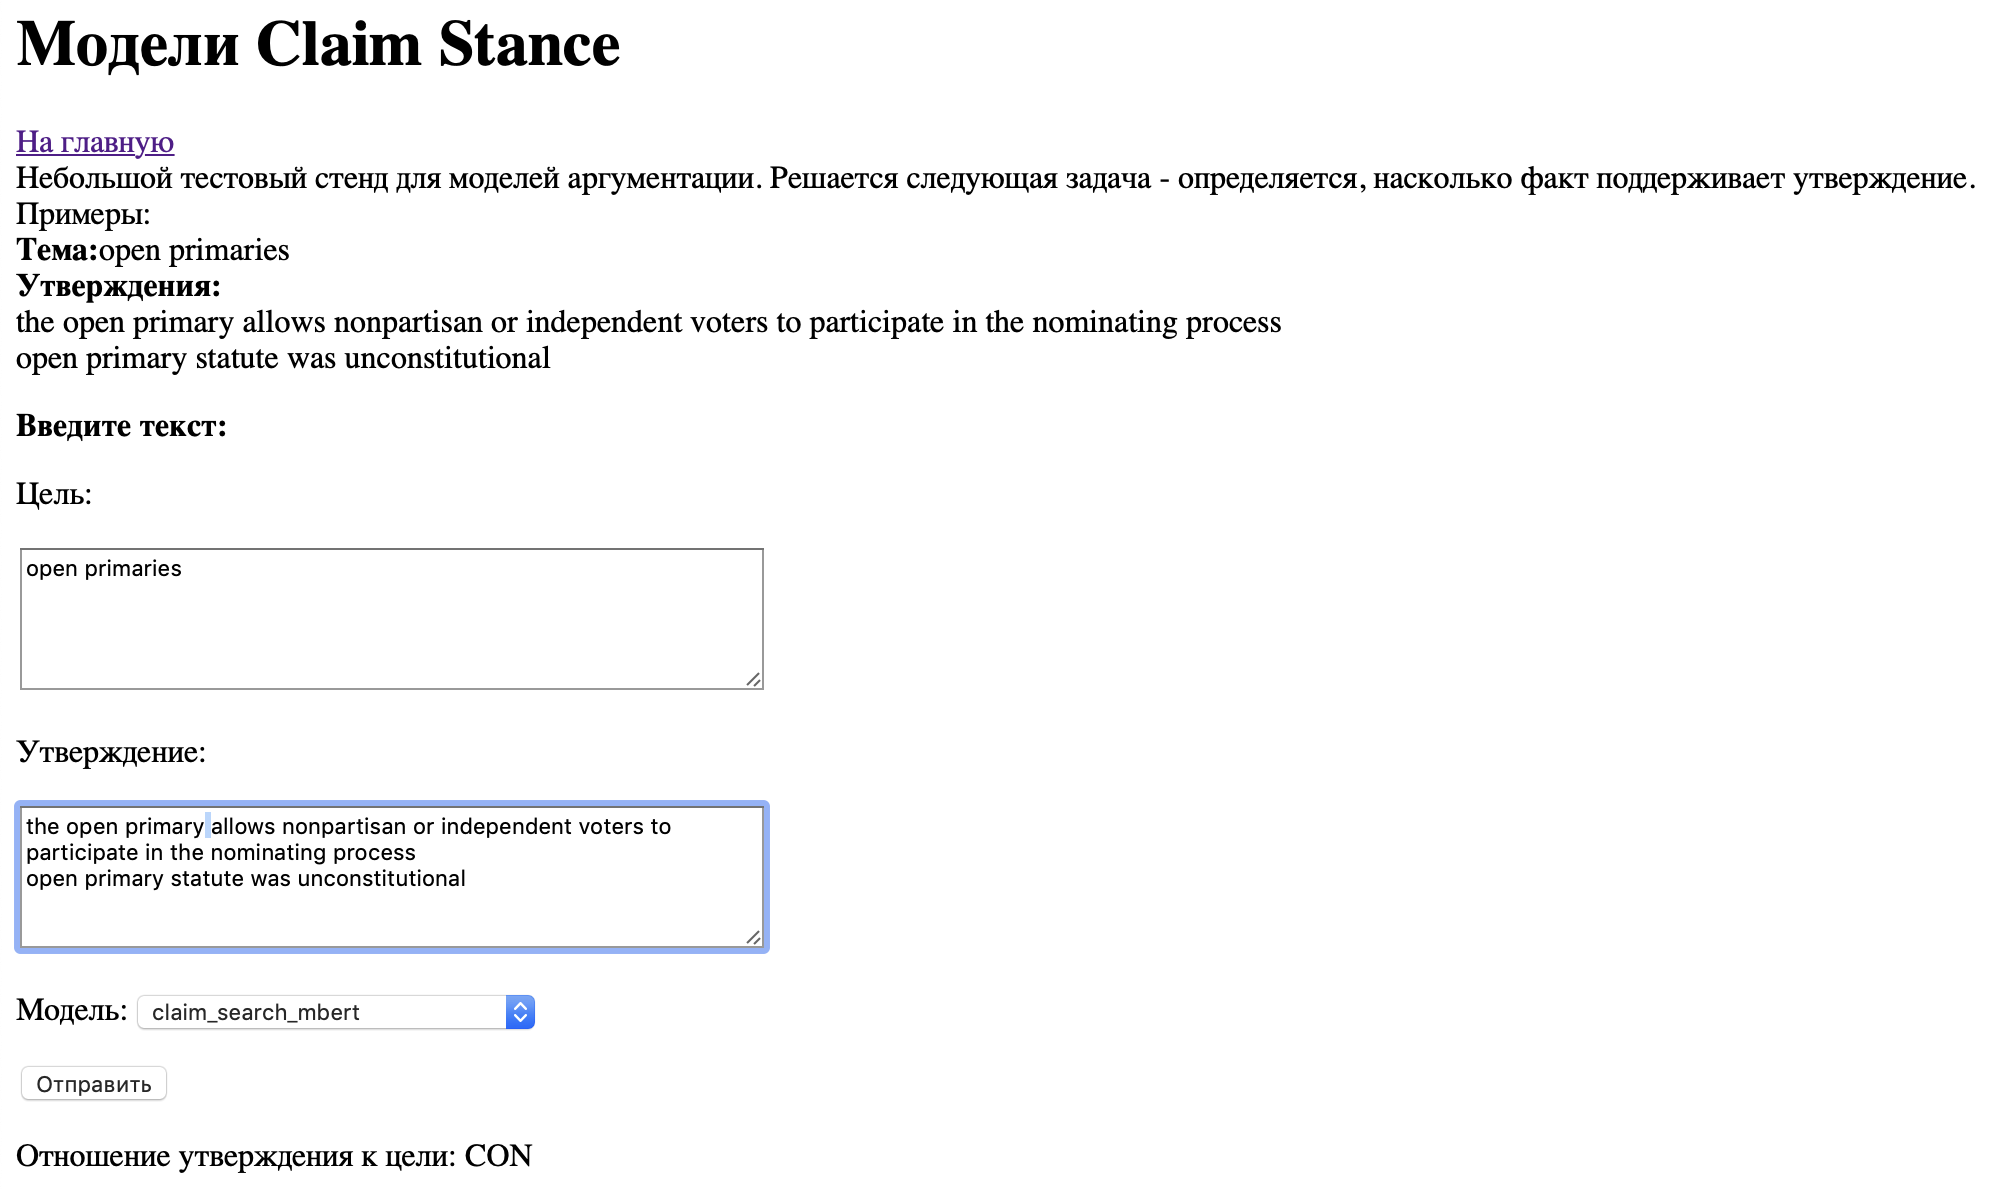
\includegraphics[scale=0.5]{service.png}}
 \caption{Интерфейс сервиса.}
\end{figure}
Для исследования эффективности работы моделей извлечения аргументации было создано веб-приложение. Веб-приложение содержит в себе 3 страницы, 2 из которых позволяют взаимодействовать с моделями.

Первая страница посвещена определению предпосылки по утверждению, а вторая страница классифицирует отношение между утверждением и предпосылкой. Каждая страница имеет 3 поля:
\begin{itemize}
    \item Поле для утверждения или темы.
    \item Поле для предпосылки.
    \item Поле для выбора моделей.
\end{itemize}

Отображение реализовано через JavaScript, поэтому результат работы модели получается без перехода на новую страницу. Для удобства анализа модели возвращается не только полученный класс связи, но также внутреннее представление модели - ее уверенность в полученном ответе.
\end{comment}